% Chapter 3

\chapter{Methodology}\label{Chapter3}

%----------------------------------------------------------------------------------------

\section{Data Description}
Data originates from a clinical neuropsychology database managed by a rehabilitation center. Raw data includes 22,075 records from 8,739 unique individuals with repeated follow-up assessments. Each assessment consists of 31 features relating to demographics/administrative details/injury specifics/neuropsychological results across six cognitive domains: Orientation/Attention/Visuospatial Perception/Language/Memory/Executive Function. Following Tier-1 filtering (described in Section~\ref{sec:filtering}), our analyzed dataset contains 17{,}406 assessments from 7{,}285 subjects.



Given that these data originate from routine clinical practice rather than a specifically constructed research protocol, test selection was influenced by both the neuropsychologist conducting testing/referral questions/patient engagement capabilities. Therefore, missingness in our dataset is structured. Certain measures appear in almost every assessment; however, some are only available in response to certain clinical circumstances. Unlike missingness originating from research protocols that may control missingness through design; missingness in this dataset varies greatly; ranging from approximately 5\% for screening tools to over 90\% for specialty assessments.



Additionally, measures fall along varying scales (standardized z-scores/scaled scores/raw timed measures). During domain aggregation (Section~\ref{sec:domain_scores}), these scales were unified. In Table~\ref{tab:missing_descriptive}, we display missingness distribution for our fourteen candidate variables. Only 53.1\% (9{,}245 assessments) of our 17{,}406 records contained complete data across all fourteen variables; if we applied listwise deletion, 46.9\% (8{,}161 assessments) of our sample could potentially be lost as a consequence of our inability to analyze this portion of our dataset. Our imputation strategy (Section~\ref{sec:imputation}) is intended to avoid losing clinical information associated with this portion of our sample.



All data have undergone deidentification according to established standards for protecting patient privacy.

\section{Tier 1 Filtering}\label{sec:filtering}
Since many variables in our dataset exhibit large amounts of missingness, we performed filtering prior to performing imputation/clustering. In general, our primary analysis employs a fifty-percent filter. Any variable that exhibits more than fifty percent missingness is eliminated; any record exhibiting more than fifty percent missingness among remaining variables is eliminated.



Our choice represents a compromise between maximizing data retention versus minimizing the amount of missingness placed on imputation models. While employing a seventy-percent filter would retain significantly more records/variables; this would increase the likelihood that artificial structure exists in our imputed data. Conversely, employing a thirty-percent filter would likely produce a clean matrix; however, it would eliminate substantially more clinically relevant records while reducing analytical capability.



We perform sensitivity analyses utilizing filters between thirty percent and seventy percent in Section~\ref{sec:robustness}.



Following application of this filter and elimination of assessments without documented cognitive testing, our dataset contains thirteen neuropsychological variables; seventeen thousand four hundred-six assessments from seven thousand two-hundred-eighty-five patients.

\begin{table}[ht]
\caption{Eligible neuropsychological variables after Tier~1 filtering, organised by cognitive domain.}
\label{tab:eligible_vars}
\centering
\small
\begin{tabular}{l p{0.55\textwidth} c}
\toprule
\textbf{Cognitive Domain} & \textbf{Variables} & \textbf{Count} \\
\midrule
Orientation        & \texttt{OPERSONA}, \texttt{OESPAI}, \texttt{OTEMPS} & 3 \\
Attention          & \texttt{ASPAN}, \texttt{ATMTA} & 2 \\
Visuoperception    & \texttt{VPIMATGES} & 1 \\
Language           & \texttt{LREPETICIOTB}, \texttt{LDENOMINACIOTB}, \texttt{LCOMPRENSIOTB} & 3 \\
Memory             & \texttt{MDIGITS}, \texttt{MRAVLT075}, \texttt{MRAVLT015}, \texttt{MRAVLT015R} & 4 \\
Executive Function & \texttt{FEPMR} & 1 \\
\midrule
\textbf{Total}     & & \textbf{14} \\
\bottomrule
\end{tabular}
\end{table}

\section{Imputation Methods}\label{sec:imputation}

The ten imputation methods compared in this dissertation are summarized in Table~\ref{tab:method_summary}. The two deep learning methods required additional training choices, so their technical details are specified here. For the denoising autoencoder (DAE), deliberately corrupted inputs were generated by masking the observed values. The corruption mask was sampled as follows:

\begin{equation}\label{eq:dae_corrupt}
\mathbf{m}_i\sim
\begin{cases}
P_{\mathrm{miss}} & \text{with probability } 0.5,\\[2pt]
\operatorname{Bernoulli}(1-\rho)^{\otimes p} & \text{with probability } 0.5,
\end{cases}
\end{equation}

where \(P_{\mathrm{miss}}\) denotes the empirical distribution of missingness patterns and \(\rho\) denotes the uniform corruption rate. This scheme allows the DAE to learn from random corruption as well as from missingness structures that resemble those observed in the clinical data.

For the variational autoencoder (VAE), cyclical annealing was used for the \(\beta\) term in the evidence lower bound. The annealing schedule was:

\begin{equation}\label{eq:beta_cyclical}
\beta(t)=\beta_{\max}\,\frac{t \bmod T}{T},\qquad T=40,\ \beta_{\max}=0.1,
\end{equation}

The deep-learning imputations were evaluated by holding out a subset \(H\) of observed entries and comparing the imputed values with the original values. Root mean square error and mean absolute error were computed as:

\begin{equation}\label{eq:rmse}
\mathrm{RMSE}=\sqrt{\frac{1}{|H|}\sum_{(i,j)\in H}\bigl(\hat{x}_{ij}-x_{ij}\bigr)^2},\qquad
\mathrm{MAE}=\frac{1}{|H|}\sum_{(i,j)\in H}\bigl|\hat{x}_{ij}-x_{ij}\bigr|.
\end{equation}

\begin{table}[htbp]
\caption{A summary of the ten imputation methods broken down by the five-category taxonomy. For clustering performance (silhouette score and number of clusters $k$) I took the best UMAP+HDBSCAN solution on the domain-level features. Note that the silhouette is on the high-density core that HDBSCAN clusters directly (before the $k$-nearest-neighbour noise-reassignment step), so it runs slightly above the final full-coverage silhouette quoted in the text (for instance MICE scores 0.598 on the core and 0.526 once every assessment is assigned; see §\ref{sec:h1_results}).}
\label{tab:method_summary}
\centering
\scriptsize
\renewcommand{\arraystretch}{1.4}
\begin{tabular}{@{} p{1.8cm} l c c c p{3.2cm} p{3cm} @{}}
\toprule
\textbf{Category} & \textbf{Method} & \textbf{Year} & \textbf{$k$} & \textbf{Sil.} & \textbf{Advantages} & \textbf{Limitations} \\
\midrule
Conventional & Mean       & ---  & 4 & 0.604 & Simplest; fast; universal baseline & Collapses variance \& covariance \\
Statistical  & EM         & 1977 & 4 & 0.587 & Principled MLE; preserves covariance & Assumes multivariate normality \\
             & MICE       & 2011 & 3 & 0.598 & Flexible; preserves distribution & Requires model per variable \\
\midrule
Machine      & KNN        & 2001 & 4 & 0.576 & Non-parametric; captures local structure & Sensitive to $k$; slow for large $n$ \\
Learning     & MissForest & 2012 & 3 & 0.606 & Non-linear; handles mixed types & Computationally expensive \\
\midrule
Hybrid       & PMM        & ---  & 4 & 0.498 & Preserves marginal distribution & Requires adequate donor pool \\
\midrule
Matrix       & SoftImpute & 2010 & 4 & 0.571 & Efficient for sparse matrices & Assumes low-rank structure \\
Completion   & NMF        & 1999 & 3 & 0.546 & Non-negativity natural for scores & Sensitive to rank choice \\
\midrule
Deep         & DAE        & 2018 & 5 & 0.510 & Non-linear; multiple imputations & Requires hyperparameter tuning \\
Learning     & VAE        & 2014 & 4 & 0.603 & Probabilistic; principled uncertainty & Complex training; $\beta$-tuning \\
\bottomrule
\end{tabular}

\vspace{0.5em}
\raggedright
\scriptsize
\textit{References:} Mean \parencite{little2019statistical}; PMM \parencite{vanbuuren2011mice}; EM \parencite{dempster1977maximum}; MICE \parencite{vanbuuren2011mice}; KNN \parencite{troyanskaya2001missing}; MissForest \parencite{stekhoven2012missforest}; SoftImpute \parencite{mazumder2010spectral}; NMF \parencite{lee1999learning}; DAE \parencite{gondara2018mida}; VAE \parencite{kingma2014auto, mccoy2018variational}.
\end{table}

\section{Domain Score Computation}\label{sec:domain_scores}
Cognitive-domain-level features were created by taking aggregated versions of variables associated with each cognitive domain while retaining the 14 individual neuropsychological variables for comparison purposes. Due to differences in scales among the original measures (e.g., standardised scores vs. scaled scores), direct aggregation would be problematic unless scale harmonization occurred. Therefore, three processing steps were taken prior to aggregation. First, each variable was winsorized to a 1st-99th percentile interval to avoid extreme imputed values caused by outliers or sentinel codes. Next, all timed tests had their signs reversed (i.e., all tests now had positive values indicating better performance). Finally, all variables were standardized to zero mean and unit variance. Reliability-weighted averages of variables representing each domain were used as domain scores. Specifically, each variable \(j\) is assigned a weight \(w_j = 1 - r_j\), where \(r_j\) represents its missingness rate. Weights are normalized within domain. Variables with greater frequency of administration therefore receive greater weighting in their respective composite scores. Reducing dimensionality from 14 individual variables to six domain-level scores provides fewer variables for distance-based algorithms to operate upon, improving geometry. Additionally, creating domain-level profiles allows clinicians to conceptualize cognitive deficits in terms of cognitive domains-rather than individual variables-making interpretation more clinically relevant. However, detail is lost. For example, two patients might have identical average memory scores yet differ in immediate versus delayed recall. Hypothesis H4 assesses whether the benefits of increased stability and interpretability provide sufficient justification for losing detail.

\section{UMAP + HDBSCAN Pipeline}\label{sec:pipeline}
Figure~\ref{fig:pipeline_diagram} shows the end-to-end process from imputed data to final cluster assignment. Prior to performing dimensional reduction using UMAP/HDBSCAN, we apply robust scaling using the median and interquartile range to reduce influence of floor and ceiling effects common in neuropsychological assessment \parencite{bellio2020analyzing,pinsky2023mad}. Floor effects occur when severely impaired patients accumulate at minimum values for an assessment tool \parencite{pinsky2023mad}, whereas ceiling effects occur when patients with no impairments accumulate at maximum values \parencite{pinsky2023mad}. Scale-free metrics like median and inter-quartile ranges help mitigate these effects. For each of the twenty imputed datasets (ten methods $\times$ two feature representations), we perform UMAP followed by HDBSCAN. Like other machine learning algorithms that rely heavily on initial conditions (in this case, random initialization), UMAP is stochastic. Therefore, a single embedding could capture variability due to either random initialization or geometric properties of the data. Therefore, we repeat each hyperparameter combination ten times and choose the embedding with highest silhouette score (based on initial HDBSCAN clustering).

\begin{figure}[htbp]
\centering
\resizebox{\textwidth}{!}{%
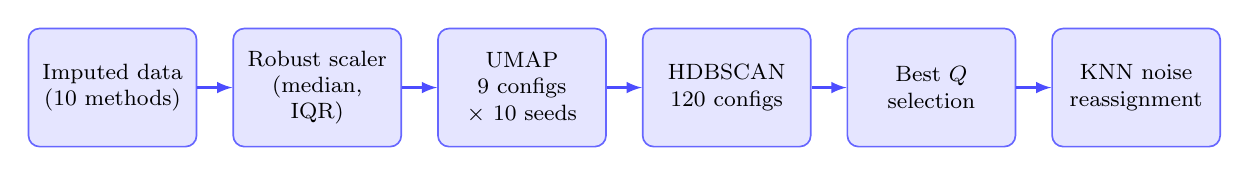
\begin{tikzpicture}[
  box/.style={draw=blue!60, line width=0.6pt, rounded corners,
              fill=blue!10, text width=1.9cm, minimum height=1.5cm,
              align=center, font=\footnotesize},
  arr/.style={->, line width=0.9pt, draw=blue!70, >=latex}
]
  \node[box] (imp) at (0,0)    {Imputed data\\(10 methods)};
  \node[box] (std) at (2.6,0)  {Robust scaler\\(median, IQR)};
  \node[box] (umap) at (5.2,0) {UMAP\\9 configs\\$\times$ 10 seeds};
  \node[box] (hdb) at (7.8,0)  {HDBSCAN\\120 configs};
  \node[box] (sel) at (10.4,0) {Best $Q$\\selection};
  \node[box] (knn) at (13.0,0) {KNN noise\\reassignment};
  \draw[arr] (imp) -- (std);
  \draw[arr] (std) -- (umap);
  \draw[arr] (umap) -- (hdb);
  \draw[arr] (hdb) -- (sel);
  \draw[arr] (sel) -- (knn);
\end{tikzpicture}%
}
\caption[Pipeline overview]{This is an end-to-end clustering pipeline. Once the data have been imputed, they first pass through a robust scaler. Next, after being scaled, the imputed data pass into a UMAP hyperparameter grid with 10 random seeds for each of nine configurations, and the resulting embeddings that yield the highest silhouette value are retained. HDBSCAN then does the clustering in a 120-configuration sweep, based upon the composite quality measure $Q = \text{silhouette} \times (1 - \text{noise fraction})$, where all boundary noise points are assigned back to their respective cluster(s) via k-nearest neighbour. This entire process is run over each of the 10 possible imputation outcomes.}
\label{fig:pipeline_diagram}
\end{figure}

\subsection{UMAP Parameter Grid}
We utilized Euclidean distance as our distance metric and \texttt{min\_dist}$=0.0$ to encourage separation between dense areas in our embedding.

\begin{table}[ht]
\caption{UMAP hyperparameter grid. All combinations of these values were put through their paces, for a total of 9 configurations.}
\label{tab:umap_grid}
\centering
\begin{tabular}{l l}
\toprule
\textbf{Parameter} & \textbf{Values} \\
\midrule
\texttt{n\_neighbors}  & 15, 30, 50 \\
\texttt{min\_dist}     & 0.0 \\
\texttt{n\_components} & 3, 5, 8 \\
\bottomrule
\end{tabular}
\end{table}

\subsection{HDBSCAN Parameter Grid}
Each UMAP embedding produced 120 possible candidate solutions (due to 120 different possible HDBSCAN configurations). To determine which configuration was "best," we employed a composite quality score that punished solutions with high silhouettes by allocating many assignments to noise:

\begin{equation}
Q = \text{silhouette} \times (1 - \text{noise proportion})
\label{eq:quality}
\end{equation}

\begin{table}[ht]
\caption{HDBSCAN hyperparameter grid. All listed value combinations were evaluated, giving me 120 configurations for each UMAP embedding.}
\label{tab:hdbscan_grid}
\centering
\begin{tabular}{l l}
\toprule
\textbf{Parameter} & \textbf{Values} \\
\midrule
\texttt{min\_cluster\_size}          & 500, 1000, 1500, 2000, 3000 \\
\texttt{min\_samples}                & 5, 10, 25, 50 \\
\texttt{cluster\_selection\_method}  & eom, leaf \\
\texttt{cluster\_selection\_epsilon} & 0.0, 0.1, 0.5 \\
\bottomrule
\end{tabular}
\end{table}

\subsection{Sweep Procedure}
The following procedures were employed for each imputed dataset: First, we preprocessed each dataset using a robust scaler. Second, we conducted a ten-fold cross-validation on each UMAP hyperparameter combination (yielding ten embeddings per combination). From these ten embeddings, we chose the best embedding based on silhouette score. Third, we conducted a 120-fold cross-validation on each HDBSCAN configuration and selected the configuration yielding the best-quality score \(Q\). Fourth, we re-labeled any observations previously labeled as noise. In doing so, noise points assigned by HDBSCAN are relocated to the nearest substantively clustered group based on k-nearest neighbor (\(k = 10\)) similarity in UMAP-space. Given that residual noise is negligible on these features, this process yields 100\% coverage and thus assigns labels to every assessment. Re-labeling is only allowed if silhouettes decrease by less than 10\%, maintaining separations between clusters.

\subsection{Worked Example}
Assume a hypothetical patient completes only those neuropsychological assessments related to orientation and digit span but fails to complete those related to Trail Making Test due to physical limitations or the delayed recall portion of the Rey Auditory Verbal Learning Test due to exhaustion. Upon application of Tier 1 filtering, however, the patient remains in the dataset with eligible variables only. The two missing scores are subsequently filled in by MICE based on observed information. The 14 variable-level scores are then subjected to winsorizing, aligned for direction, standardized, and weighted as defined in Section~\ref{sec:domain_scores} to produce six domain-composite scores. The robust scaler is applied to minimize the effect that floor and ceiling effects may have on aggregate measures. The resulting six-dimensional vector is then mapped into the cohort's UMAP representation space. The patient is then classified into one of three cognitive-severity tiers: Above Average, Near Normal, or Globally Impaired. If a patient falls into a sparse area of low density and was classified as noise, KNN reassignment utilizes neighboring assessments in UMAP-space (\(k = 10\)) and assigns them to the most closely located substantively-clustered tier. The final output includes a tier label and confidence score based on how often each imputation method agrees under hypothesis H2.

\section{Hypothesis Definitions}\label{sec:hypotheses}
\noindent \textbf{H1 (Existence of Cognitive Clusters)}. The UMAP + HDBSCAN pipeline will likely find at least two distinct, stable cognitive clusters for most imputation techniques. The existence of these clusters can be demonstrated as long as the best solution from at least 8 of the 10 different methods has both characteristics: average silhouette $\geq$ 0.40 and percentage of noisy points \(< 0.30\). Since we allow some method-specific failures, the 80\% criterion provides a margin for error.



\noindent \textbf{H2 (Robustness Across Imputation Techniques)}. Solutions for the clustering problems should show reasonable to high agreement among the imputation methods. H2 is confirmed if the median pairwise ARI and NMI for each of the $\binom{10}{2} = 45$ combinations of methods exceeds 0.50. Although there is considerable flexibility in setting this threshold, it is greater than chance and implies a substantial overlap in group membership, regardless of the degree to which individual solutions are identical.



\noindent \textbf{H3 (Relationship Between Clinical Unit \& Cluster Membership)}. Cluster membership is expected to be related to clinical unit. For each imputation technique, a contingency table is created and a chi-square test of independence is conducted. H3 is confirmed if the relationship remains statistically significant at \(\alpha = 0.05\) after a Bonferroni adjustment and Cramér's \(V > 0.10\). As a sensitivity check for potential confounds, a Cochran-Mantel-Haenszel (CMH) test is performed, conditioned on an appropriate covariate.



\noindent \textbf{H4 (Clustering at Domain-Level vs. At Variable Level)}. I expect the cognitive features at the domain level to result in a clustering representation that is more interpretable and at least as well separated as the representation based on cognitive features at the variable level. H4 will be confirmed if the domain-level approach performs at least as well as or better than the variable-level approach on at least two of three metrics: (1) higher silhouette scores; (2) lower mean VIFs; and (3) lower condition numbers. Smaller values of VIF and condition number imply less multicollinearity and better numerical conditioning. Because cross-method agreement has already been assessed in H2, comparisons of feature representations are made in H4 exclusively.

\section{Statistical Tests and Validation}\label{sec:stats}

\subsection{Statistical Conventions}
Each statistical evaluation of hypotheses follows typical statistical practice. Each evaluation assesses the data relative to a null hypothesis \(H_0\), representing a "no-effect" baseline. The p-value is the probability of obtaining a test statistic as extreme as that obtained assuming \(H_0\) to be true; smaller p-values represent stronger evidence against \(H_0\). A predetermined significance level of \(\alpha = 0.05\) serves as the threshold for rejecting \(H_0\). For any parameter, a 95\% CI represents the range that would include the population parameter in 95\% of repeated random samples from the same population using the same methodology.



For applications of bootstrapping, observed data are randomly sampled with replacement to generate a simulated approximation of the sampling distribution of a statistic. The 2.5th and 97.5th percentiles of that simulated distribution define the bootstrap CI. A z-score quantifies how many standard deviations away from the mean of a specified reference distribution a given value lies. With respect to the psychological testing instruments employed here, standardized testing permits scores derived from different instruments to be compared.



Cohen defined standards for interpreting the magnitude of effects, specifically for standardized differences, i.e., Cohen's \(d\). Specifically, \(d = 0.20\) is interpreted as a small effect size, \(d = 0.50\) as a medium-sized effect, and \(d = 0.80\) as a large effect size. When applying Cramér's V as an effect size for evaluating chi-squared tests, \(V = 0.10\) is interpreted as a small effect size, \(V = 0.30\) as a medium effect size, and \(V = 0.50\) as a large effect size.

\begin{equation}\label{eq:cohend}
d=\frac{\bar{x}_1-\bar{x}_2}{s_p},\qquad s_p=\sqrt{\frac{(n_1-1)s_1^2+(n_2-1)s_2^2}{n_1+n_2-2}},
\end{equation}

\subsection{Tests and Validation Procedures}
\noindent \textbf{Bootstrap Stability}. I conduct a bootstrap stability analysis for every imputation method using \(B = 50\) resamplings. For each resampling, I refit HDBSCAN on the cached UMAP embeddings, recording the median silhouette (Eq.~\ref{eq:silhouette}) and pre-KNN noise proportions. Pre-KNN noise proportion is equal to the proportion of observations that do not belong to any meaningful cluster:

\begin{equation}\label{eq:noise}
\text{noise}=\frac{1}{n}\bigl|\{\,i:\text{label}(i)=\text{noise}\,\}\bigr|,
\end{equation}

This is also the value used in defining quality function \(Q\) (Eq.~\ref{eq:quality}). According to H1's pre-defined conditions, a method will be deemed successful if its median silhouette is larger than or equal to 0.40 and its pre-KNN noise proportion is less than or equal to 0.30; at least 8 of the 10 methods will need to satisfy both conditions. To evaluate per-cluster stability, I apply Hennig (2007)'s matching algorithm to the pre-KNN labels using the default threshold (i.e., 0.7).



\noindent \textbf{Pairwise Agreement}. In order to remove imputation-induced variability caused by variations in other parts of pipelines, I employ a shared pipeline strategy. One StandardScaler, one UMAP model, and one k-means model are trained on MICE-imputed domain scores. The remaining methods are then standardized, projected onto this MICE-trained pipeline, and classified using that same MICE-trained pipeline. This creates the ARI (Eq.~\ref{eq:ari}) and NMI (Eq.~\ref{eq:nmi}) matrices comparing each method to each other shown as heatmaps in Chapter~\ref{Chapter4}. Confidence for each assessment is defined as:

\begin{equation}\label{eq:consensus}
\mathrm{conf}(i)=\max_{\ell}\frac{1}{M}\sum_{m=1}^{M}\mathbf{1}\!\left[\text{label}_m(i)=\ell\right],
\end{equation}

High-confidence assessments are those whose assessments were placed into the mode cluster by at least \(M/10 = 0.8 \times 10 = 8\) methods.



\noindent \textbf{Chi-Square Test, Cramér's V, CMH Test}. Contingency tables arise from cross-classifying two categorical variables - e.g., cluster assignment and clinical unit - giving joint counts. Pearson's Chi-Square Test evaluates observed counts \(O_{ij}\) against expected counts \(E_{ij}\) under the null hypothesis that the two variables are independent:

\begin{equation}\label{eq:chi2}
\chi^2=\sum_{i=1}^{r}\sum_{j=1}^{c}\frac{(O_{ij}-E_{ij})^2}{E_{ij}},\qquad E_{ij}=\frac{O_{i\cdot}\,O_{\cdot j}}{n},
\end{equation}

with \(O_{i\cdot}\) and \(O_{\cdot j}\) denoting row sums and column sums, respectively. The test statistic is referenced against a Chi-Square distribution with \((r - 1)(c - 1)\) degrees of freedom to yield the p-value. Cramér's V is used to render association statistics scale-free for sample-size purposes, since it takes on values between zero and one:

\begin{equation}\label{eq:cramersv}
V=\sqrt{\frac{\chi^2}{n\,(k-1)}},\qquad k=\min(r,c),
\end{equation}

The Cochran-Mantel-Haenszel Test extends Pearson's Chi-Square Test for data organized into strata (e.g., diagnosis subgroups). The CMH Test determines whether the association between cluster assignments and clinical units remains significant even when stratifying by an appropriate covariate:

\begin{equation}\label{eq:cmh}
\chi^2_{\mathrm{CMH}}=\frac{\bigl(\sum_{h}(a_h-\mathbb{E}[a_h])\bigr)^2}{\sum_{h}\operatorname{Var}(a_h)}.
\end{equation}



\noindent \textbf{Variance Inflation Factor}. To quantify multicollinearity in regression models, VIF is used. For any variable \(j\), it is defined as:

\begin{equation}\label{eq:vif}
\mathrm{VIF}_j=\frac{1}{1-R_j^2},
\end{equation}

where \(R_j^2\) denotes the coefficient of determination when regressing \(j\) on all other predictors. Any value exceeding 10 constitutes grounds for concern, and influences interpretation both at the variable level and in subsequent analyses at the domain level.

\subsection{Implementation}

\begin{sloppypar}
All analyses were implemented in Python (version 3.13).
Imputation used
\texttt{scikit-learn} (KNN, NMF),
\texttt{fancyimpute} (SoftImpute, EM),
\texttt{miceforest} (MICE, PMM), and
\texttt{missforest} (MissForest).
DAE and VAE used \texttt{PyTorch}.
UMAP used \texttt{umap-learn};
HDBSCAN used the \texttt{hdbscan} library.
Statistical tests used \texttt{scipy.stats} and \texttt{statsmodels}.
Validation metrics used \texttt{scikit-learn}.
The full source code, notebooks, and dashboard are available at
\url{https://github.com/zkunos/thesis_project}.
\end{sloppypar}

%----------------------------------------------------------------------------------------
